
\section{Logical layer}
\label{logical}
This layer represents the outermost level of abstraction, where information is handled and manipulated at a software level.
For a transmitter, the processes included in this layer regard the input of the message from a user, its encoding and communication to the control layer.
Most importantly, for a receiver module the logical layer handles the interpretation of data from the sensor back into an encoded message with meaning, its decoding and finally the presentation of the information to its final consumer.
Additionally, the logical layer is responsible of improving the reliability of the system where possible, with control mechanisms that add robustness to the unreliable aspects of the communication.
A good logical layer could handle recovery techniques in cases where symbols are missing or mistaken, and overall reduction of noise impact. 
For instance the implementation of a basic communication protocol could help in making the communication more stable and structured, allowing elementary operations such as checking correctness and encapsulation.
The complexity of the transmitter logical layer is not particularly high, the layer takes some message as input, manipulates it to meet the encoding and protocol requirements and redirects it to the control layer. 
The focus of this section will therefore be shifted to the receiving side of the communication.
The requirements that the logical layer is expected to meet are that the communication rate is not significantly slowed down by the software processes, and that communication is successfully achieved.
This final objective particularly relies on the signal recognition on the reception side.
 
\begin{figure}[htbp]
   \centering
   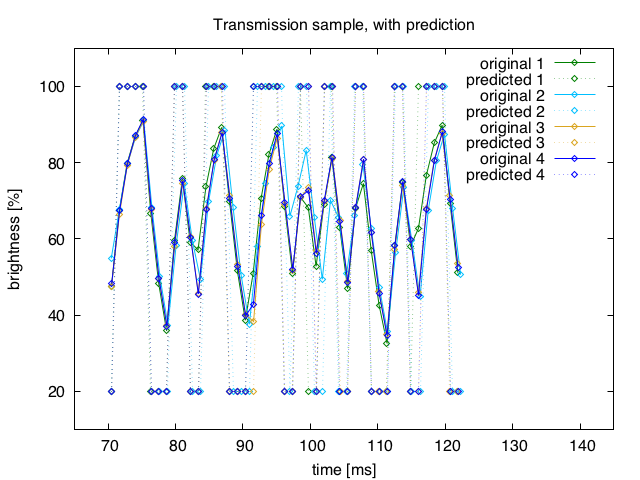
\includegraphics[height=200px]{img/sample} 
   \caption{Example of the results of interpreting digital information from analog input.}
   \label{fig:sample}
\end{figure}

%reading 
 \subsection{Reading the signal}
A key part of this layer is to convert analog sensor data representing light variations into binary code.
Fig. \ref{fig:sample} shows a sample of transmission.
The full lines, predominantly blue in the central part of the figure, represent the values registered by the sensor, while the dotted lines at the top and bottom represent a reconstruction of the digital signal.
When the analog signal comes as a sequence of increasing values, the digital prediction of the signal is  a 1, and when the sequence of values is decreasing, the prediction is set to 0.
%The green line represents the original values from the light sensor, while the purple line is a reconstruction of what the digital transmission would look like. 
Manchester encoding allows transmission to only have two kinds of peak, either representing single symbols, like a 1 or a 0, or two symbols of the same kind, like a 11 or a 00.
This is because each binary 1 is represented as the sequence 01, and each 0 as 10.
Whenever two subsequent bits are different, there will be a sequence of two symbols of the same kind in Manchester encoding.
As an example, the sequence 0 0 0 0 0 0 1 0, representing the byte 0x02, would be encoded as 10 10 10 10 10 10 01 10.
When there is the switch between a binary 0 and ta binary 1, a sequence of two 0 symbols appear in the Manchester encoded byte.
During transmission this would graphically translate to a longer and deeper 0 symbol in the reception.
The same discussion applies in reverse for a double 1.
Luckily, longer same symbol sequences are not possible with this encoding.\\
The design of an algorithm that could go through these sequences of sensory values and interpret them into binary data has undergone through different stages and different attempts.

\subsubsection{Machine Learning approach}
The first version of an algorithm for prediction made use of Machine Learning techniques to predict digital symbols given sequences of sensor data.
These techniques include the training of a model with training data, that would "teach" a classifier what kinds of sequences produce given results.
 The training data was taken in different circumstances of ambient light interference, with different messages sent and at different times.
Multiple classifiers were tested, with a maximum success rate of about 75\% of correct predictions. 
The classifiers included NaiveBayes, RandomForest, AdaBoost and ArtificialNeuralNetworks, all with comparable results.\\
There were major difficulties with this approach. 
To begin with, there were problems identifying the labels to train these models with, namely the classes or categories where the data would belong.
Initially, the four categories were "1", "0", "11", and "00". The basic idea is that given a sequence of values, its corresponding digital symbol should fall in one of these four classes.
A problem in implementing this approach was that single symbols and double symbols have sequences of values from the sensor of different sizes. 
These sizes are also called the number of features for a machine learning sample.\\
The standard module for machine learning that was used requires the same number of features for all the labels.\\
Given this restriction, the labels became "10", "01", "11", and "00". Eventually, also these labels were produced by different numbers of features, at times. Other combinations were tried, and eventually all leading to the same result. 
One way to get around this problem is to have a fixed number of features, but big enough to include all the possibilities. 
Samples smaller than this maximum amount (eventually all of the samples) would be filled up with blank values until they reach the intended size.\\
Another way would be to train a classifier for each specific number of features that may occur. In this case, the amount of classifiers needed would have been around 4, for number of features ranging between 7 and 10 with a transmission rate of 500 Hz.
The downside of this approach is that each classifier becomes very specific to a restricted set of the training data, potentially loosing track completely of certain labels.\\
The final setup for machine learning prediction used the labels "101", "100", "011", "110", "001", "11", "00", "10", "01", scaling of the features and larger sample size to be filled up with blanks.
This produced overall the best results for the machine learning approach, but never above 80\% success rate.\\
A downside to this final approach would be that when receiving values from the sensor in real time, a moving window  of the fixed size of the number of features would be necessary, and an attempt of prediction should be made at every new value inserted.
This might likely slow down the reading process.
Otherwise, it would also be necessary to keep track of the variations to only attempt a prediction when there is a switch in direction and the sequence is within a desired length.
These additional control techniques would minimise the purpose of machine learning altogether, suggesting that only keeping track of the values could be sufficient to produce a prediction.

\subsubsection{Custom algorithm approach}
These poor results ultimately led to a change of approach for reading the data, guided by the continuous adjustments performed on the previous approach. 
Just looking at fig. \ref{fig:sample} it is immediately evident that the high peaks represent 1s and the low peaks represent 0s. 
By setting some rules, a custom classifier could predict a result for a sequence of values without even the need to be trained with sample data.
In particular, the classifier analyses sequences of values, trying to find sequences that are either monotonically increasing or monotonically decreasing.
Also a noise factor has to be taken into account, in this way small enough variations are not considered.
As mentioned before, there are only two kinds of peaks in the sequences, either single or double peaks, due to the encoding of the signal.
Therefore, it is of critical importance to be able to distinguish the two cases. One criteria that was originally deployed for this was to count the number of values that progress in the same direction, either up or down. 
This was later changed to the more precise criteria of duration of such sequences, and for this reason for each sensor value a timestamp is also included in the control layer, representing the time of reception for that specific value.\\ 
With this in mind, the algorithm has been developed to very simply count the duration of either monotonically increasing or decreasing sequences of values, and produce a prediction when the direction changes, based on such duration.
This technique performs particularly well in this application, producing up to 100\% success rate in optimal conditions.
 Runtime wise, the algorithm takes constant time for each value that is received, and may or may not produce a resulting prediction.
A simplified version of the algorithm can be found in fig. \ref{code}, written in Python 2.7.\\
One aspect that is of crucial importance is the parameter called \_$doubletime$ in the code.
This parameter represents the level above which the duration of a signal is considered a double symbol.
With a continuous reception and optimal conditions, this value would be exactly the interval of time that two subsequent symbols last in the transmitter.
For a transmission rate of 500 Hz, with intervals of 2 ms between two signals, two subsequent symbols would last exactly 4 ms.
However, setting the parameter to be 4 ms would produce wrong results in many cases, due to the reception rate.
A reception rate of 1200 Hz produces a reading every approximately 0.833 ms, which means that a 4 ms interval would fall between four received values after 3.332 ms, and five received values after 4.165 ms.
In many cases, the fifth value received after 4.165 ms from the start of the sequence is already the first step to the opposite direction, therefore the sequence lasts 1 sample value less.
This is why the parameter \_$doubletime$ needs to be adjusted according to the reception rate and not the transmission rate, in this example at 3.332 ms instead of 4 ms.

\subsection{Protocol}
As can be seen the rates of transmission and reception in this prototype system are not very high, if compared to average wireless transmission speeds, which are measured in Mbps.
Transmission in visible light is also exposed to a high degree of uncertainty, depending on parameters like distance, maximum brightness, interference, noise, and so on.
In this prototype, communication is only established in one direction, which additionally increases the threat of getting wrong results.
In order to compensate all these aspects, an effort to strengthen the success rate has been made by structuring the communication into a very basic protocol.
Each message is therefore encapsulated into a Protocol Data Unit, or PDU.
Each PDU is enclosed between two single bytes: a byte STX, that indicates the start of a message, and a byte ETX which indicates its end. 
These two are bytes 0x02 and 0x03 respectively.
To avoid that the receiver wrongfully interprets an ETX byte while reading the message, perhaps as a combination of the final part of one byte and the start of another, a length byte LEN is also included in the header of the PDU, to specify the length of the message in bytes.
Additionally, each PDU is restrained to have a maximum size, and longer messages need to be split into more PDUs.
This is mostly to preserve the serial connection between logical layer and control layer, to avoid overflow of the serial buffer.
This three fields combined should make it adequately easy for the receiver to know if some parts of the message were lost during transmission.
Since the communication is established mono-directionally, the transmitter wouldn't know if the message was delivered, but the receiver most likely would.
Mistaken symbols are very unlikely in this kind of communication, it is much more likely to entirely miss some.
Therefore the receiver could easily know if the message was delivered or not, by comparing the length of the message that was initially declared and the length of the message that was received.
To increase the chances of a successful delivery, the transmitter could be transmitting the same message over and over in a mono-directional scenario.

\subsubsection{Additional fields}
Increasing the functionalities or complexity of the system, additional parameters in the PDU might result useful if not necessary. 
Imagining a scenario with multiple receivers of messages broadcasted through light in a unilateral way, a receiver ID field could be added to the PDU.
 Also, it would be wise to perform encryption on the PDUs, in a way that only the intended receivers would be able to read the message directed to them.
Establishing 2-way communication would also require more steps.
In a 2-way communication it would be much easier to ensure correctness of the transmission. 
For this, at least 2 more parameters seem necessary: a sequence number to identify the packet, and a checksum to check correctness of the received message.
When the message received is of a different length than declared or produces a different checksum, the receiving side of the communication could just ask  for the same message again, or confirm correct reception otherwise.
A header for visible light communication doesn't require many parameters in the case where a system establishes only local communication.
Otherwise for messages to travel through a network, a PDU header would also need routing parameters for origin and destination of the message.

\begin{figure}
\centering
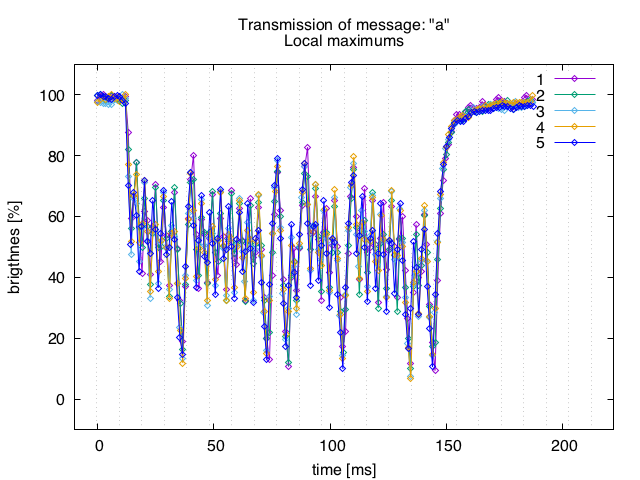
\includegraphics[height=180px]{img/transmission}
\caption{Example of transmission of message "a", the transmission include STX, ETX, and LEN bytes, over 5 samples.}
\label{fig:transmissionA}
\end{figure}

\subsection{Result}
Figure \ref{fig:transmissionA} shows an example of the transmission of the message "a", including STX, ETX and LEN bytes.
In the figure it can be seen that the transmission starts from 100\% of brightness, and returns to 100\% when it is finished. 
This is the normal operation of the communication system.
With this approach, although the rate of transmission is still fast enough to not be perceived by human eye, the perception of the light intensity drops to about 60\% during communication, as an average of high and low peaks.
This makes it possible to actually guess when there is transmission just by observing the light.
A different approach could be to keep alternating 1s and 0s even when there is no message to send, or to reduce the light intensity to a similar level during non-transmission.\\
Other than knowing when there is transmission just by observing the light intensity, it is impossible to decode the message without recurring to machines.
Once the signal as it is received is displayed graphically however, the traits of the signal in the figure can be visually associated with the Manchester encoding of the message, clearly visible at least in the occurrence of double symbols. \\
In ASCII, letter "a" is represented by the byte 0x61, or 01100001 in binary and 97 as decimal.
As previously mentioned, the STX is byte 0x02, ETX byte 0x03, and LEN in this case would be 1.
In binary, the entire message would then be: 00000010 - 00000001 - 01100001 - 00000011, as STX-LEN-"a"-ETX.\\
In Manchester encoding: 10101010101\textbf{0011}0 - 1010101010101\textbf{001 - 100}10\textbf{11}010101\textbf{001 - 1}0101010101\textbf{00}101.
A 00 and a 11 are clearly visible at the end of the first byte in the figure, at about 40 ms after the start of the sample.
 A 00 almost concludes the second byte at around 70 ms in the figure, follows a 11 connecting the second to the third byte, then a 00, 11, and so on.
 This feature of the communication also allows manual debugging during the development process.
  \todo{protocol vs no protocol?}

\subsubsection{Experimental evaluation}
To test performance of the communication in its final stage, multiple tests have been performed on the prototype.
For each test, the system takes user input for initialising the message to send, encodes it and sends it through light. 
The receiver reconstructs the message depending on values retrieved from the sensor.
Tests have been performed at very close proximity of the sensor to the light source, without other lights directly facing the sensor but with presence of natural light.
A test is considered successful if every bit is correctly received and interpreted.
Messages of different sizes have been tested.
Table \ref{tab:txresults} illustrates the results of these tests.
The message length reported on the table is measured in characters of the payload, each character represented by one byte and 16 symbols in Manchester encoding.
For each message the 3 control bytes STX, LEN, ETX are also sent and need to be added for the total length of the message.
%
\begin{table}[hbt]
\centering
  \begin{tabular}{l c c c c c}
    distance & message length (chars) & symbols in pdu &  ambient light & tests & successful \\
    \hline
   0 cm & 5 & 128 & yes & 50 & 100\% \\
   0 cm & 10 & 208 & yes & 50 & 100\% \\
   0 cm & 20 & 368 & yes & 50 & 100\% \\
   0 cm & 30 & 528 & yes & 50 & 100\% \\
   10 cm & 5 & 128 & yes & 50 & 92\% \\
   10 cm & 10 & 208 & yes & 50 & 96\% \\
   10 cm & 20 & 368 & yes & 50 & 88\% \\
   10 cm & 30 & 528 & yes & 50 & 60\% \\
  \end{tabular}
  \caption{Tests of full transmission, success criteria is 100\% correctness.}
  \label{tab:txresults}
\end{table}
%
From to these results, it is possible to calculate the probability of receiving a symbol successfully at a distance of 10 cm.
Assuming the event of receiving a symbol correctly is independent from the reception of previous symbols, the probability of receiving $x$ symbols correctly becomes $P(x) = P(1)^x$, where $P(1)$ represents the probability of receiving one symbol correctly. 
Given $P(x)$ as the probability reported on the table, this makes the probability of receiving a single symbol correctly $P(1) = \sqrt[x]{P(x)}$.
According to the results, this value ranges between $0.99903..$ and $0.99980..$ .
These results also confirm that shorter messages have a greater probability of being interpreted correctly, which makes the enforcement of the maximum PDU length rule even more important.

\begin{figure}
\centering
\begin{lstlisting}[language=Python, frame={}]
	def feed(self, time, value):
		pred = None
		
		# staying
		if abs(value - self.prev) <= self.epsilon:
			pass

		#going down
		elif value <= self.prev: 
			if self.direction: # up	
				pred = self._predict(time)

		# going up
		elif value > self.prev: 
			if not self.direction: # down
				pred = self._predict(time)

		self.prev = value
		return pred
		
	def _predict(self, time):
		m = self.direction
		delta = time - self.seqstart
		pred = '-'
		
		if delta >= self._doubletime:
			pred = '11' if m else '00'
		else:
			pred = '1' if m else '0'

		self.direction = not self.direction
		self.seqstart = time
		return pred
\end{lstlisting}
\caption{Simplified algorithm for signal interpretation (Python 2.7).}
\label{code}
\end{figure}